%%%%%%%%%%%%%%%%%%%%%%%%%%%%%%%%%%%%%%%%%%%%%%%%%%%%%%%%%%%%%%%%%%%%%%%%%%%
%
% Plantilla para un artículo en LaTeX en español.
%
%%%%%%%%%%%%%%%%%%%%%%%%%%%%%%%%%%%%%%%%%%%%%%%%%%%%%%%%%%%%%%%%%%%%%%%%%%%

% Qué tipo de documento estamos por comenzar:
\documentclass[a4paper]{article}
% Esto es para que el LaTeX sepa que el texto está en español:
\usepackage[spanish]{babel}
\selectlanguage{spanish}
% Esto es para poder escribir acentos directamente:
\usepackage[utf8]{inputenc}
\usepackage[T1]{fontenc}



%% Asigna un tamaño a la hoja y los márgenes
\usepackage[a4paper,top=3cm,bottom=2cm,left=3cm,right=3cm,marginparwidth=1.75cm]{geometry}

%% Paquetes de la AMS
\usepackage{amsmath, amsthm, amsfonts}
%% Para añadir archivo∫s con extensión pdf, jpg, png or tif
\usepackage{graphicx}
\usepackage[colorinlistoftodos]{todonotes}
\usepackage[colorlinks=true, allcolors=blue]{hyperref}


%% Primero escribimos el título
\title{Problema de la Satisfacibilidad Booleana}
\author{Fernanda Domínguez Acosta, Ximena Sandoval del Hoyo, Raúl Murcia Yocupicio}
}

%% Después de "preámbulo", podemos empezar el documento

\begin{document}
%% Hay que decirle que incluya el título en el documento
\maketitle

%% Iniciamos "secciones" que servirán como subtítulos

\section{Definiciones}

\subsection{Definición de la Clase NP}

aaaaaaaaaaaaaaaaaaaaaaaaaaaaaaaaa
aaaaaaaaaaaaaaaaaaaaaaaaaaaaaaaaa


aaaaaaaaaaaaaaaaaaaaaaaaaaaaaaaaa

aaaaaaaaaaaaaaaaaaaaaaaaaaaaaaaaa
aaaaaaaaaaaaaaaaaaaaaaaaaaaaaaaaa


aaaaaaaaaaaaaaaaaaaaaaaaaaaaaaaaa
aaaaaaaaaaaaaaaaaaaaaaaaaaaaaaaaa



\subsection{Reducciones en tiempo polinomial}
Nuestra principal metodología para probar que un problema $P_2 \notin \mathcal{P}$
es la reducción de un problema $P_1$, sabiendo que $P_1 \notin \mathcal{P}$, a $P_2$.

\begin{figure}[h]
\centering
\graphicspath{ {./Images/} }
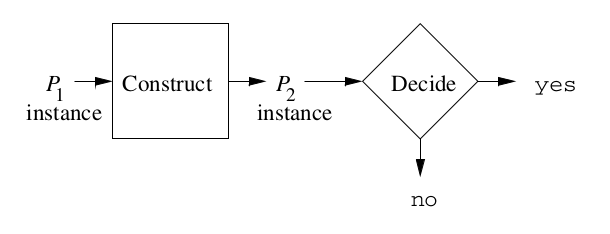
\includegraphics[width=0.5\textwidth]{reduccion.png}
\caption{\label{fig:Reduccion}Esquema de reducción\cite{hopcroft2001introduction}}
\end{figure}
Sin embargo, la existencia de un algoritmo llamado ``Construct'' no es suficiente
para probar ``Si $P_1$ no está en $\mathcal{P}$ entonces $P_2$ tampoco está en $\mathcal{P}$''.

Supongams que dada una instancia de $P_1$ de longitud $m$, podemos encontrarnos
con dos situaciones:
\begin{itemize}
  \item El algoritmo de construcción produce una cadena de salida con longitud $2^{m}$, que entra en el hipotético algoritmo polinomial de $P_2$. Si este algoritmo toma un tiempo $\mathcal{O}(n^k)$ entonces con una cadena de longitud $2^{m}$ tomará un tiempo $\mathcal{O}(2^{km})$, exponencial sobre $m$.
  \item El algoritmo de construcción produce una cadena de salida con longitud $m$ pero toma un tiempo exponencial en ello, como $\mathcal{O}(2^m)$. Ahora el algoritmo de decisión para $P_2$ toma un tiempo polinomial $\mathcal{O}(n^k)$ para una entrada de tamaño $n$ pero el algoritmo de decisión para $P_1$ toma $\mathcal{O}(2^{m} + m^{k})$.
\end{itemize}
Estos hechos implican que $P_1 \notin \mathcal{P}$ y $P_2 \in \mathcal{P}$

La restricción correcta para una construcción de $P_1$ a $P_2$ es que requiere
un tiempo polinomial sobre el tamaño de la entrada.
Esto implica que dicha construcción toma un tiempo $\mathcal{O}(m^{j})$ es un
cadena de longitud $m$, por lo que la instancia de $P_2$ no puede ser mayor al
número de pasos que tomó, es decir, a lo más $cm^{j}$ para una constante $c$.
Con esto podemos probar que si $P_2 \in \mathcal{P}$ entonces $P_1 \in \mathcal{P}$.

Supongamos que podemos decidir si una cadena de longitud $n$ pertenece a $P_2$
en un tiempo $\mathcal{O}(n^{k})$. Entonces podemos probar si una cadena de
longitud $m$ pertenece a $P_1$ en un tiempo $\mathcal{O}(m^j + (cm^j)^k)$,
donde $m^j$ cuenta el tiempo del algoritmo de construcción y $(cm^j)^k$ el
tiempo para decidir si el resultado de la construcción pertenece a $P_2$.
Notamos que al simplificar el tiempo para $P_1$ obtenemos
$\mathcal{O}(m^j + (cm^{jk})$, donde $c$, $j$ y $k$ son constantes, por lo que
el tiempo es polinomial sobre $m$, por lo que podemos concluir que $P_1 \in \mathcal{P}$.

\subsection{Definición de la Clase NP-Completo}

AAAAAAAAAAAAAAAAAAAAAAAAAAAAAAA

\section{El problema de satisfacibilidad}
%Descripción
El problema de la satisfacibilidad booleana es un problema NP-completo\cite{cook1971complexity}.



\subsection{Codificación del problema}

Las variables se identifican con

\section{Demostración}
Para demostrar que SAT es NP-Completo, primero tenemos que demostrar que es de la clase NP.

\subsection{SAT pertenece a la clase NP}
así es

\subsection{SAT pertenece a la clase NP-Completo}


% Ejemplo de figurita que puede ayudar después
%\begin{figure}
%\centering
%\includegraphics[width=0.5\textwidth]{tesla.jpg}
%\caption{\label{fig:tesla}Esta imagen se añadió en el menú Project.}
%\end{figure}


\bibliographystyle{plain}
\nocite{*}
\bibliography{main}

% Nota
%Para las bibliografías está rotísimo, para que salga todo hay que hacer:
% pdflatex main.tex -f
% bibtex main
% pdflatex main.tex -f
% pdflatex main.tex -f
%
% Dos veces al final

\end{document}
